\documentclass[conference]{IEEEtran}
\IEEEoverridecommandlockouts
\usepackage{cite}
\usepackage{amsmath,amssymb,amsfonts}
\usepackage{algorithm}
\usepackage{algorithmic}
\usepackage{graphicx}
\usepackage{textcomp}
\usepackage{xcolor}
\usepackage{booktabs}

\begin{document}

\title{Federated Learning in SDVs: Optimizing Communication Frequency}

\author{\IEEEauthorblockN{Spyridon Arvanitis}
\IEEEauthorblockA{\textit{Department of Informatics and Telematics} \\
\textit{Harokopio University of Athens}\\
Athens, Greece}
}

\maketitle

\begin{abstract}
Deploying Federated Learning (FL) on Software-Defined Vehicles (SDVs) involves balancing wireless transmission overhead, client model divergence, and onboard compute contention with safety-critical vehicular workloads. Existing vehicular FL frameworks typically assume dedicated onboard compute and rely on static local training schedules, which frequently leads to uplink channel congestion and compute starvation for co-located real-time services. In this paper, we propose a runtime heuristic policy engine that dynamically regulates local training epochs and client upload schedules based on available compute slack, instantaneous link throughput, and predicted local learning gain. The engine formalizes a three-state execution model (\texttt{WAIT}, \texttt{CONTINUE}, \texttt{SYNC}) and uses bounded non-linear curve fitting to extrapolate empirical loss trajectories before committing onboard execution slack. We evaluate the approach across Dirichlet non-IID partitioned benchmarks ($\alpha_{\text{Dir}} \in \{0.1, 0.3, 0.5\}$) under realistic V2X channel traces against static epoch baselines ($E \in \{1, 5, 10\}$) and FedProx over 250 communication rounds. Under severe statistical skew ($\alpha_{\text{Dir}} = 0.1$), the dynamic policy attains 70.29\% top-1 centralized test accuracy with FedAvg and 72.51\% with FedProx, outperforming high-epoch static training ($68.87\%$). Furthermore, the engine reduces cumulative uplink bandwidth consumption by 34.5\% (saving over 8.0~GB of wireless transfers), eliminates 83.2\% of transmission buffer dropouts (down from 567 to 95), and reduces compute contention on safety-critical tasks by up to 60.7\%.
\end{abstract}

\begin{IEEEkeywords}
Federated Learning, Software-Defined Vehicles, V2X Networks, Resource Allocation, Mixed-Criticality Systems.
\end{IEEEkeywords}

\section{Introduction}
Modern Software-Defined Vehicles (SDVs) operate as mobile computing platforms running complex machine learning workloads for driver assistance, cabin perception, and vehicular diagnostics. Because these systems continuously generate substantial volumes of high-dimensional sensor data, Federated Learning (FL) provides an attractive paradigm for collaboratively training shared models across fleets without transferring raw, privacy-sensitive telemetry to cloud infrastructure.

However, executing FL in vehicular networks introduces operational constraints that differ fundamentally from conventional edge computing environments:
\begin{enumerate}
    \item \textbf{Dynamic V2X Link Contention:} Vehicle-to-Everything (V2X) wireless links exhibit time-varying channel attenuation, handovers, and limited cell uplink capacity. Synchronizing high-dimensional parameter updates across multiple vehicles during each communication round rapidly congests local cellular infrastructure. Conversely, artificially reducing synchronization frequency over heterogeneous (non-IID) vehicular data induces severe model divergence (client drift), degrading global convergence.
    \item \textbf{Mixed-Criticality Hardware Contention:} SDVs rely on consolidated, virtualized hardware architectures where FL workloads must share CPU and accelerator capacity with safety-critical Electronic Control Unit (ECU) services (e.g., ADAS perception, object tracking, and trajectory planning). In-vehicle FL is strictly a secondary background process that must yield execution slack whenever safety-critical processes demand compute. Enforcing static training schedules without inspecting processor occupancy risks severe compute starvation and deadline misses for higher-priority tasks.
\end{enumerate}

Existing vehicular FL scheduling solutions generally focus on link-level optimization, rate adaptation, or joint transmit-power allocation while treating onboard compute as either fixed or dedicated. A crucial limitation is the absence of \emph{learning-aware} decision making: current frameworks determine upload frequency and client selection based on channel conditions and computational budgets, but never evaluate whether the local training they schedule produces meaningful model improvements. Under non-IID vehicular data, a client may reach diminishing returns after two local epochs, yet a fixed-epoch policy forces it to continue---wasting compute, increasing parameter drift, and degrading convergence upon aggregation. A second gap concerns mixed-criticality hardware contention: existing formulations model onboard compute as unlimited or statically partitioned, ignoring the time-varying nature of safety workload demand. When an ADAS perception pipeline experiences a transient spike, a scheduler that continues training can induce deadline violations in safety-critical tasks.

To address these combined operational challenges, we propose an online runtime policy engine that coordinates compute allocation, local training depth, and upload decisions via a unified utility maximization objective:
\begin{equation*}
\max \sum \left[ \delta \cdot G_i(t) - \alpha C_{\text{net}}(t) - \beta C_{\text{comp}}(t) - \gamma C_{\text{drift}}(t) \right]
\end{equation*}
Rather than assuming dedicated hardware, our engine monitors co-located workload occupancy, channel capacity, and model divergence to dynamically transition clients among three discrete execution states: \texttt{WAIT} (idle and yield compute), \texttt{CONTINUE} (autonomous local training with weight persistence), and \texttt{SYNC} (parameter upload). In particular, the explicit \texttt{WAIT} state prevents vehicles from burning energy or contending with ADAS tasks when channel throughput is low and anticipated learning gain is negligible.

The main contributions of this work are:
\begin{itemize}
    \item We formulate the vehicular FL scheduling problem as an online utility maximization framework that jointly optimizes empirical learning gain against uplink bandwidth penalties, safety-critical compute contention, and parameter drift.
    \item We develop a three-state runtime policy engine (\texttt{WAIT}, \texttt{CONTINUE}, \texttt{SYNC}) that incorporates bounded non-linear exponential curve fitting to predict marginal validation gain before executing subsequent local epochs.
    \item We validate the mechanism on non-IID Dirichlet-partitioned vehicular testbeds ($\alpha_{\text{Dir}} \in \{0.1, 0.3, 0.5\}$) against static epoch baselines ($E \in \{1, 5, 10\}$) and FedProx across 250 communication rounds, demonstrating a 34.5\% reduction in pure uplink bandwidth (17.3\% total payload), an 83.2\% reduction in transmission buffer dropouts (from 567 to 95), and up to 60.7\% lower compute contention against safety-critical vehicle tasks.
\end{itemize}

\section{Related Work}
Vehicular federated learning literature can be broadly categorized into three primary domains: mobility-aware transmission scheduling, joint compute-communication optimization, and model compression frameworks.

\subsection{Mobility-Aware Transmission Scheduling}
Several studies focus on wireless channel uncertainty and vehicle mobility. Hong et al.~\cite{ref_hong} modeled Vehicle-to-Infrastructure (V2I) model uploads as a Markov Decision Process (MDP) to reduce latency and power consumption. Karatas et al.~\cite{ref_karatas} proposed variable-rate client selection to mitigate imperfect channel state information. Yan et al.~\cite{ref_yan} introduced opportunistic Vehicle-to-Vehicle (V2V) relays to facilitate model transfers under energy constraints. These methods address link degradation but treat vehicular compute capacity as an unconstrained or static parameter.

\subsection{Joint Compute and Communication Co-Design}
To address the coupling between onboard execution time and wireless transmission delay, joint resource allocation frameworks have been explored. Qiang et al.~\cite{ref_qiang} investigated dynamic model partitioning across vehicular edge nodes based on instantaneous processor and bandwidth availability. Ballotta et al.~\cite{ref_ballotta} proposed a predictive computation-scheduling method using radio environment maps. Zhang et al.~\cite{ref_zhang_selection} jointly optimized client selection and resource allocation to improve convergence accuracy, while Pervej et al.~\cite{ref_pervej} formulated iteration counts and CPU frequencies alongside physical resource block allocations. Li et al.~\cite{ref_fedprox} introduced FedProx to introduce a proximal regularization term that handles system and statistical heterogeneity. Although these formulations link computation latency with transmission budgets, they generally assume dedicated hardware partitions for FL.

\subsection{Compressed and Asynchronous Frameworks}
To reduce communication bottlenecks and handle stragglers, quantization and asynchronous aggregation have been deployed. Liu et al.~\cite{ref_liu} optimized local batch sizes and gradient compression ratios under latency bounds. Zhang et al.~\cite{ref_zhang_quant} evaluated adaptive quantization schemes based on channel conditions. In asynchronous settings, Wu et al.~\cite{ref_wu} tuned upload frequency to instantaneous link quality, and Zhang et al.~\cite{ref_zhang_automotive} deployed sliding-window parameter transfers on embedded automotive GPUs.

\begin{table*}[t]
\caption{Comparison of Vehicular FL Resource Allocation Approaches}
\label{tab:related_work}
\centering
\begin{tabular}{lp{4.2cm}p{4.2cm}p{4.5cm}}
\toprule
\textbf{Reference} & \textbf{Compute Modeling} & \textbf{Network Modeling} & \textbf{Optimization Objective} \\
\midrule
Hong et al.~\cite{ref_hong} & Implicit / fixed execution latency & Uplink transmit power and duration & Minimize weighted upload delay and energy \\
Karatas et al.~\cite{ref_karatas} & Uniform client processing rate & Imperfect CSI, adaptive transmission rate & Accelerate convergence under link uncertainty \\
Yan et al.~\cite{ref_yan} & Static local compute baseline & V2V/V2I relay and opportunistic links & Maximize upload success probability \\
Qiang et al.~\cite{ref_qiang} & CPU frequency and split layers & Dynamic channel bandwidth & Minimize total processing and transmission delay \\
Ballotta et al.~\cite{ref_ballotta} & Local iteration scheduling & Radio environment maps, path loss & Optimize training progress under round deadlines \\
Zhang et al.~\cite{ref_zhang_selection} & General compute resource bounds & Channel-aware client selection & Maximize final model accuracy \\
Pervej et al.~\cite{ref_pervej} & CPU frequency and iteration bounds & PRB allocation, sojourn time & Joint energy-delay trade-off under mobility \\
Liu et al.~\cite{ref_liu} & Batch size scaling & Gradient compression ratio, spectrum allocation & Maximize convergence rate under delay caps \\
Zhang et al.~\cite{ref_zhang_quant} & Latency-coupled computation & Multi-level parameter quantization & Trade off quantization error and latency \\
Wu et al.~\cite{ref_wu} & Adaptive local training loops & Asynchronous upload scheduling & Minimize transmission redundancy \\
Zhang et al.~\cite{ref_zhang_automotive} & Embedded GPU hardware evaluation & Sliding-window parameter exchange & Asynchronous convergence on embedded systems \\
\textbf{Proposed} & \textbf{Dynamic safety workload occupancy ($U_i^{\text{crit}}$)} & \textbf{Time-varying cell capacity and throughput} & \textbf{Joint utility maximization: learning gain vs. bandwidth, model drift, and compute contention} \\
\bottomrule
\end{tabular}
\end{table*}

\subsection{Summary and Positioning}
As summarized in Table~\ref{tab:related_work}, existing approaches primarily optimize radio resource blocks or static computation partitions. Critically, no prior work jointly evaluates: (i)~\emph{whether} an additional local epoch will produce measurable learning gain, and (ii)~\emph{whether} the vehicle's CPU can afford that epoch without starving co-located safety workloads. Modern SDVs operate in mixed-criticality environments where FL shares compute capacity with high-priority safety tasks. Our work bridges both gaps by introducing a dynamic compute occupancy metric ($U_i^{\text{crit}}(t)$), a bounded exponential gain predictor, and an online heuristic that co-optimizes training depth and communication timing based on real-time vehicle resource constraints and empirical learning dynamics.

\section{System Model and Problem Formulation}
We consider a vehicular federated learning network with $N$ client vehicles, indexed by $\mathcal{V} = \{1, 2, \dots, N\}$, communicating with an edge or roadside server over discrete decision rounds $t \in \{0, 1, \dots, T-1\}$.

\subsection{Vehicle State Representation}
At round $t$, each vehicle $i \in \mathcal{V}$ observes a local state vector:
\begin{equation}
S_i(t) = \{B_i(t),\, U_i^{\text{crit}}(t),\, D_i(t),\, G_i^{\text{prior}}(t)\}
\end{equation}
where:
\begin{itemize}
    \item $B_i(t)$ represents the instantaneous uplink bandwidth available to vehicle $i$ (in Mbps).
    \item $U_i^{\text{crit}}(t) \in [0, 1]$ denotes the fraction of onboard compute capacity occupied by safety-critical tasks (e.g., ADAS perception and trajectory planning).
    \item $D_i(t)$ indicates client model drift relative to the latest global model parameters.
    \item $G_i^{\text{prior}}(t)$ denotes the historical empirical learning gain achieved during the vehicle's preceding active training window.
\end{itemize}

\subsection{Cost and Gain Formulation}
The operational metrics governing training round $t$ are formalized as follows:

\subsubsection{Communication Cost}
Let $p_i(t) \in \{0, 1\}$ denote the binary transmission decision ($p_i(t) = 1$ indicates model upload). The network transmission delay penalty is modeled as:
\begin{equation}
C_{\text{net}}(t) = \sum_{i \in \mathcal{V}} p_i(t) \frac{M_i}{B_i(t)}
\end{equation}
where $M_i$ is the physical parameter payload size in megabytes (e.g., 9.31~MiB for an FP32 ResNet-9 model).

\subsubsection{Compute Contention Cost}
Let $c_i(t) \in [0, 1]$ represent the normalized compute allocation granted to the FL process ($c_i(t) = e_i(t)/\rho_i$, where $e_i(t)$ is the executed local epochs and $\rho_i$ is the maximum epoch capacity). The contention penalty imposed on co-located services is defined as:
\begin{equation}
C_{\text{comp}}(t) = \sum_{i \in \mathcal{V}} c_i(t) U_i^{\text{crit}}(t)
\end{equation}

\subsubsection{Parameter Divergence (Model Drift)}
We measure client drift $D_i(t)$ directly as the true global parameter vector Euclidean distance between local parameters $\mathbf{w}_{\text{local}, i}(t)$ and received global parameters $\mathbf{w}_{\text{global}}(t)$:
\begin{equation}
D_i(t) = \| \mathbf{w}_{\text{local}, i}(t) - \mathbf{w}_{\text{global}}(t) \|_2 = \sqrt{\sum_{l=1}^L \| \mathbf{w}_{i, l}(t) - \mathbf{w}_{\text{global}, l}(t) \|_2^2}
\end{equation}
where $l \in \{1, \dots, L\}$ indexes all weight and bias tensors. The cumulative fleet drift is:
\begin{equation}
C_{\text{drift}}(t) = \sum_{i \in \mathcal{V}} D_i(t)
\end{equation}

\subsubsection{Learning Gain and Marginal Utility}
To quantify empirical optimization progress, we track local validation loss reduction:
\begin{equation}
G_i(t) = \max\left(0,\, L_i(\mathbf{w}_{\text{global}}(t)) - L_i(\mathbf{w}_{\text{local}, i}(t))\right)
\end{equation}
At local epoch $e \in \{1, \dots, \rho_i\}$, the client evaluates the marginal utility of executing epoch $e+1$:
\begin{equation}
\Delta U_i(e+1) = \delta \cdot \widehat{G}_i(e+1) - \beta \frac{U_i^{\text{crit}}(t)}{\rho_i} - \gamma D_i(e+1)
\label{eq:marginal_utility}
\end{equation}
where $\widehat{G}_i(e+1)$ is the expected loss reduction predicted via curve fitting, and $\delta, \beta, \gamma$ are positive weighting coefficients.

The marginal utility $\Delta U_i(e{+}1)$ serves as a per-epoch decision criterion that enables fine-grained adaptive training depth. Rather than committing to a predetermined number of local epochs, each vehicle evaluates whether the expected improvement in validation loss outweighs the resource costs. This prevents two failure modes inherent in fixed-epoch FL: (i)~\emph{under-training}, where clients with rich local datasets are artificially limited; and (ii)~\emph{over-training}, where clients with depleted or redundant data continue burning compute and accumulating destructive drift.

\subsection{Global Fleet Optimization Objective}
The global fleet objective over time horizon $T$ is formulated as an online utility maximization:
\begin{equation}
\max_{\{c_i(t), e_i(t), p_i(t)\}} \sum_{t=0}^{T-1} \left[ \delta \sum_{i \in \mathcal{V}} G_i(t) - \alpha C_{\text{net}}(t) - \beta C_{\text{comp}}(t) - \gamma C_{\text{drift}}(t) \right]
\label{eq:global_opt}
\end{equation}

The positive term $\delta \sum_i G_i(t)$ rewards measurable empirical progress, while the penalty terms impose costs for bandwidth consumption, safety-critical compute contention, and parameter divergence. This structure ensures that the trivially cost-optimal solution of not training is penalized by forfeiting learning rewards, while the trivially gain-optimal solution of unrestricted training is penalized by resource costs. The policy engine therefore seeks the productive equilibrium between learning progress and operational sustainability.

\noindent subject to:
\begin{align}
& c_i(t) \le 1 - U_i^{\text{crit}}(t), \quad \forall i, t \label{eq:slack_constraint} \\
& e_i(t) \le \rho_i c_i(t), \quad \forall i, t \label{eq:epochs_constraint} \\
& \sum_{i \in \mathcal{V}} p_i(t) M_i \le B_{\text{cell}}(t), \quad \forall t \label{eq:cell_constraint} \\
& D_i(t) \le D_i^{\text{max}}, \quad \forall i, t \label{eq:drift_constraint}
\end{align}

Constraint~\eqref{eq:slack_constraint} restricts FL execution to available compute slack. Constraint~\eqref{eq:epochs_constraint} bounds local training epochs by available compute. Constraint~\eqref{eq:cell_constraint} limits simultaneous uploads to total cell uplink capacity $B_{\text{cell}}(t)$, and~\eqref{eq:drift_constraint} bounds client parameter deviation.

Because future channel throughput and safety workload spikes are non-deterministic, solving~\eqref{eq:global_opt} offline is intractable. We implement an online deterministic policy engine that approximates this objective at each decision interval.

\section{Runtime Policy Engine}

\begin{algorithm}[t]
\caption{Dynamic Runtime Policy Engine for FL Vehicle $i$}
\label{alg:policy_engine}
\begin{algorithmic}[1]
\REQUIRE State $S_i(t)$, local model $\mathbf{w}_i$, thresholds $\{B_{\text{thresh}}, G_{\text{thresh}}, \tau_{\text{continue}}, D_i^{\text{max}}\}$, compute ceiling $\rho_i$, weights $\{\delta, \beta, \gamma\}$.
\STATE $c_i^{\text{max}} \leftarrow \max(0, 1 - U_i^{\text{crit}}(t))$
\IF{$c_i^{\text{max}} < 1 / \rho_i$}
    \RETURN \texttt{WAIT} ($e_i \leftarrow 0, p_i \leftarrow 0$) \COMMENT{Safety workload starvation}
\ENDIF
\IF{$B_i(t) < B_{\text{thresh}}$ \AND $G_i^{\text{prior}} \le G_{\text{thresh}}$}
    \RETURN \texttt{WAIT} ($e_i \leftarrow 0, p_i \leftarrow 0$) \COMMENT{Poor channel, low utility}
\ENDIF
\STATE Initialize $e \leftarrow 0$, history $H \leftarrow [L_i(0)]$
\WHILE{$(e + 1)/\rho_i \le c_i^{\text{max}}$ \AND $e < \rho_i$}
    \STATE Execute 1 local epoch on $\mathbf{w}_i$
    \STATE $e \leftarrow e + 1$; measure $L_i(e)$
    \STATE Smooth: $L_{\text{smooth}} \leftarrow \theta L_i(e) + (1-\theta) H[\text{last}]$; append to $H$
    \IF{$e < 2$}
        \STATE \textbf{continue}
    \ENDIF
    \STATE Extrapolate $\widehat{L}(e+1) \leftarrow \text{BoundedExpFit}(H)$
    \STATE $\widehat{G} \leftarrow \max(0, H[\text{last}] - \widehat{L}(e+1))$
    \STATE $D_i \leftarrow \| \mathbf{w}_i - \mathbf{w}_{\text{global}} \|_2$
    \STATE $\Delta U \leftarrow \delta \widehat{G} - \beta (U_i^{\text{crit}} / \rho_i) - \gamma D_i$
    \IF{$D_i > D_i^{\text{max}}$ \OR $\widehat{G} < G_{\text{thresh}}$ \OR $\Delta U < \tau_{\text{continue}}$}
        \STATE \textbf{break}
    \ENDIF
\ENDWHILE
\STATE $G_i^{\text{actual}} \leftarrow \max(0, L_i(0) - L_i(e))$; $G_i^{\text{prior}} \leftarrow G_i^{\text{actual}}$
\IF{$e = 0$ \OR ($B_i(t) < B_{\text{thresh}}$ \AND $G_i^{\text{actual}} \le G_{\text{thresh}}$)}
    \RETURN \texttt{WAIT} ($e_i \leftarrow 0, p_i \leftarrow 0$)
\ENDIF
\IF{$B_i(t) \ge B_{\text{thresh}}$}
    \RETURN \texttt{SYNC} ($e_i \leftarrow e, p_i \leftarrow 1$) \COMMENT{Upload model update}
\ELSE
    \RETURN \texttt{CONTINUE} ($e_i \leftarrow e, p_i \leftarrow 0$) \COMMENT{Retain weights locally}
\ENDIF
\end{algorithmic}
\end{algorithm}

At each decision round $t$, each client evaluates local constraints and transitions among three discrete execution states (detailed in Algorithm~\ref{alg:policy_engine}):

\begin{itemize}
    \item \textbf{WAIT (Idle):} The vehicle performs zero local epochs ($e_i=0$) and transmits no update ($p_i=0$). This state is entered under two conditions: (i) compute slack is insufficient for even a single epoch ($1 - U_i^{\text{crit}} < 1/\rho_i$), yielding CPU capacity to safety tasks; or (ii) uplink throughput is degraded ($B_i < B_{\text{thresh}}$) while prior learning progress is negligible ($G_i^{\text{prior}} \le G_{\text{thresh}}$). This prevents energy waste and model drift when transmission is infeasible and training yields diminishing returns.
    \item \textbf{CONTINUE (Autonomous Local Training):} When compute slack permits but the uplink channel is congested ($B_i < B_{\text{thresh}}$), yet local loss is actively decreasing ($G_i > G_{\text{thresh}}$), the vehicle continues training locally without uploading ($p_i=0$). Crucially, client weights are preserved across rounds rather than reset to global weights, allowing autonomous multi-epoch optimization.
    \item \textbf{SYNC (Model Upload):} When local training concludes and instantaneous link throughput satisfies $B_i(t) \ge B_{\text{thresh}}$, the client uploads its updated parameter vector ($p_i=1$). The server incorporates the update into federated aggregation and updates the global model.
\end{itemize}

\subsection{Bounded Exponential Gain Prediction}
To decide whether committing computational slack to epoch $e+1$ yields positive marginal utility, the client fits an exponential parametric curve to observed validation loss history:
\begin{equation}
L(e) \approx L_\infty + A e^{-B e}
\end{equation}
Unconstrained non-linear regression on short, noisy loss trajectories ($N \ge 3$) frequently suffers from numerical instability, producing negative asymptotic losses ($L_\infty < 0$) or negative decay rates ($B < 0$). To guarantee well-behaved predictions, we formulate a bounded non-linear least squares optimization:
\begin{equation}
\min_{L_\infty, A, B} \sum_{k=0}^{e} \left( L(k) - (L_\infty + A e^{-B k}) \right)^2
\end{equation}
subject to $0 \le L_\infty \le \min(H)$, $A \ge 0$, and $10^{-4} \le B \le 10.0$, solved with initial estimate $p_0 = [0.8 \min(H),\, H[0] - 0.8\min(H),\, 0.5]$. If numerical convergence is not achieved within 1,500 iterations, the engine defaults to a robust linear-slope decay fallback:
\begin{equation}
\widehat{L}(e+1) = \max\left(0,\, L(e) + 0.5 \cdot (L(e) - L(e-1))\right)
\end{equation}
This bounded design prevents premature policy abortion and ensures stable convergence.

\section{Performance Evaluation}

\subsection{Experimental Setup}
The evaluation testbed is implemented using PyTorch and the Flower federated learning framework. The client workload uses a ResNet-9 architecture modified with Group Normalization (8 groups) across convolutional stages to mitigate running-statistic divergence under non-IID data partitioning. Training is conducted on the CIFAR-10 benchmark distributed over $N = 10$ vehicular clients using symmetric Dirichlet partitioning ($\alpha_{\text{Dir}} \in \{0.1, 0.3, 0.5\}$) to simulate extreme to moderate non-IID statistical heterogeneity.

The evaluation benchmarks include:
\begin{itemize}
    \item Static FedAvg baselines with fixed local epochs $E \in \{1, 5, 10\}$.
    \item Fixed FedProx ($E = 5, \mu = 0.01$) to assess proximal regularization against client drift.
    \item The proposed Dynamic FL policy (FedAvg and Dynamic FedProx) operating with calibrated coefficients: $\alpha = 0.005$, $\beta = 1.0$, $\gamma = 0.006$, $\delta = 27.0$, $B_{\text{thresh}} = 20.0$~Mbps, and $G_{\text{thresh}} = 0.01$. These weights were selected by extracting non-dominated solutions along the empirical Pareto frontier of an offline 100-trial hyperparameter sweep (shown in Fig.~\ref{fig:pareto_frontier}).
\end{itemize}
Network traces and vehicular workload occupancy $U_i^{\text{crit}}(t)$ are driven by empirical V2X channel datasets, with total cell uplink capacity modeled as a dynamic sinusoidal envelope ($B_{\text{cell}}(t) = B_{\text{max}}(0.8 + 0.2\sin(t))$) to assess performance under shared infrastructure bottlenecks.

\begin{figure*}[t]
\centering
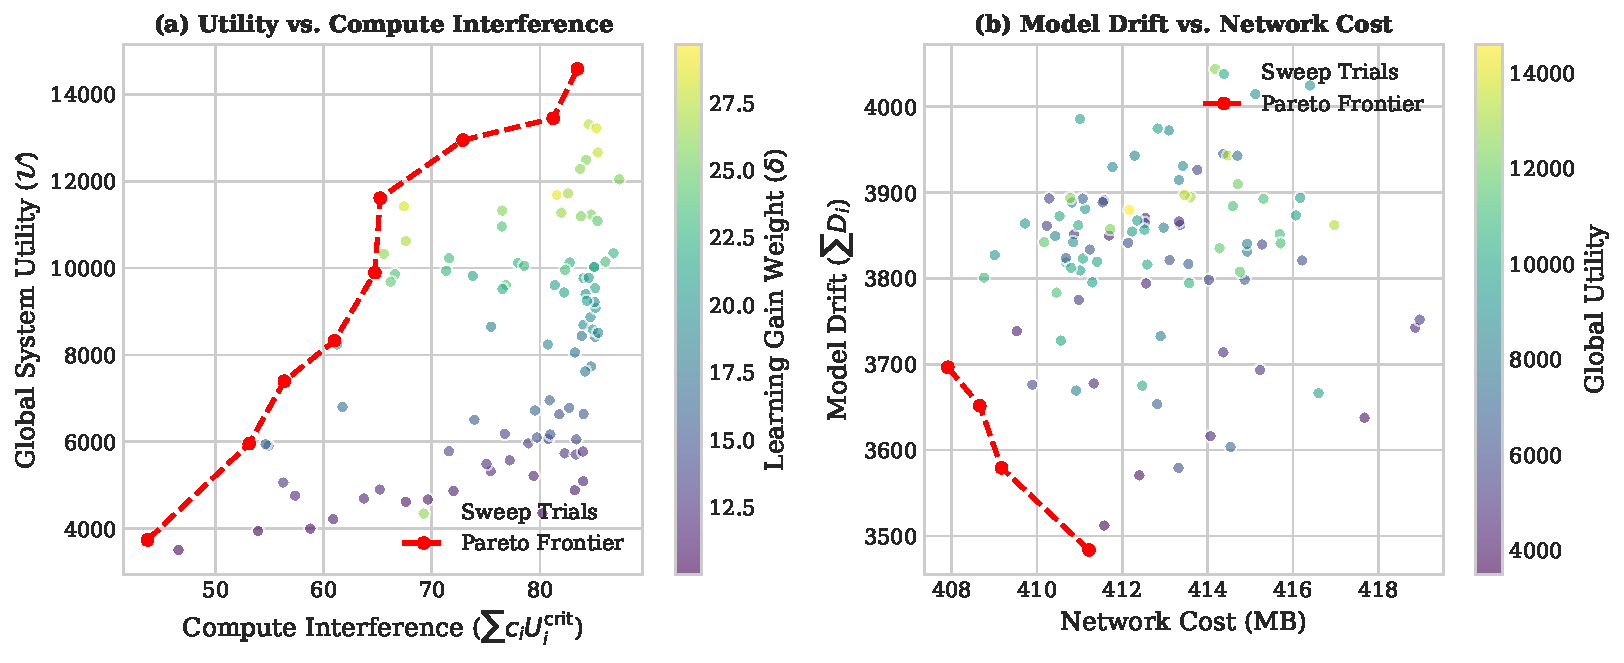
\includegraphics[width=0.92\linewidth]{plots/pareto_frontier_tradeoffs.pdf}
\caption{Empirical Pareto frontiers extracted from a 100-trial offline hyperparameter sweep: (a) Global system utility ($\mathcal{U}$) vs. compute contention ($\sum c_i U_i^{\text{crit}}$) colored by learning gain weight $\delta$; (b) Model drift ($\sum D_i$) vs. cumulative network cost (MB) colored by utility. Dashed red curves identify non-dominated Pareto configurations utilized to calibrate operational engine weights.}
\label{fig:pareto_frontier}
\end{figure*}

\begin{table*}[t]
\caption{Comprehensive Benchmark Results Across Non-IID Dirichlet Partitions (250 Communication Rounds)}
\label{tab:evaluation_results}
\centering
\begin{tabular}{lccccccr}
\toprule
\textbf{Policy / Scheme} & \multicolumn{3}{c}{\textbf{Centralized Test Accuracy (\%)}} & \textbf{Cumulative Uplink} & \textbf{Upload} & \textbf{Compute Contention} & \textbf{Parameter Drift} \\
 & $\alpha = 0.1$ & $\alpha = 0.3$ & $\alpha = 0.5$ & \textbf{Payload (MB)} & \textbf{Drops} & \textbf{Cost ($\sum c_i U_i^{\text{crit}}$)} & \textbf{Cost ($\sum D_i$, $\alpha=0.1 / 0.5$)} \\
\midrule
Fixed FedAvg ($E = 1$) & 71.09 & 77.00 & \textbf{78.84} & 23,272.2 & 567 & 100.1 & 3,635.2 / 2,977.9 \\
Fixed FedAvg ($E = 5$) & \textbf{72.93} & \textbf{77.63} & 78.14 & 23,272.2 & 567 & 500.3 & 4,202.7 / 2,417.8 \\
Fixed FedAvg ($E = 10$) & 68.87 & 77.50 & 78.26 & 23,272.2 & 567 & 1,000.6 & 4,309.7 / 2,474.4 \\
Fixed FedProx ($E = 5, \mu = 0.01$) & 70.81 & 77.35 & 78.64 & 23,272.2 & 567 & 500.3 & 2,949.2 / 2,056.0 \\
\textbf{Dynamic FedAvg (Ours)} & 70.29 & 76.51 & 78.21 & \textbf{15,238.6} & \textbf{95} & 381.6--393.0 & 3,986.0 / 2,773.9 \\
\textbf{Dynamic FedProx (Ours)} & 72.51 & 76.79 & 78.17 & \textbf{15,238.6} & \textbf{95} & 373.0--398.5 & \textbf{2,541.1 / 2,038.3} \\
\bottomrule
\end{tabular}
\end{table*}

\begin{figure*}[t]
\centering
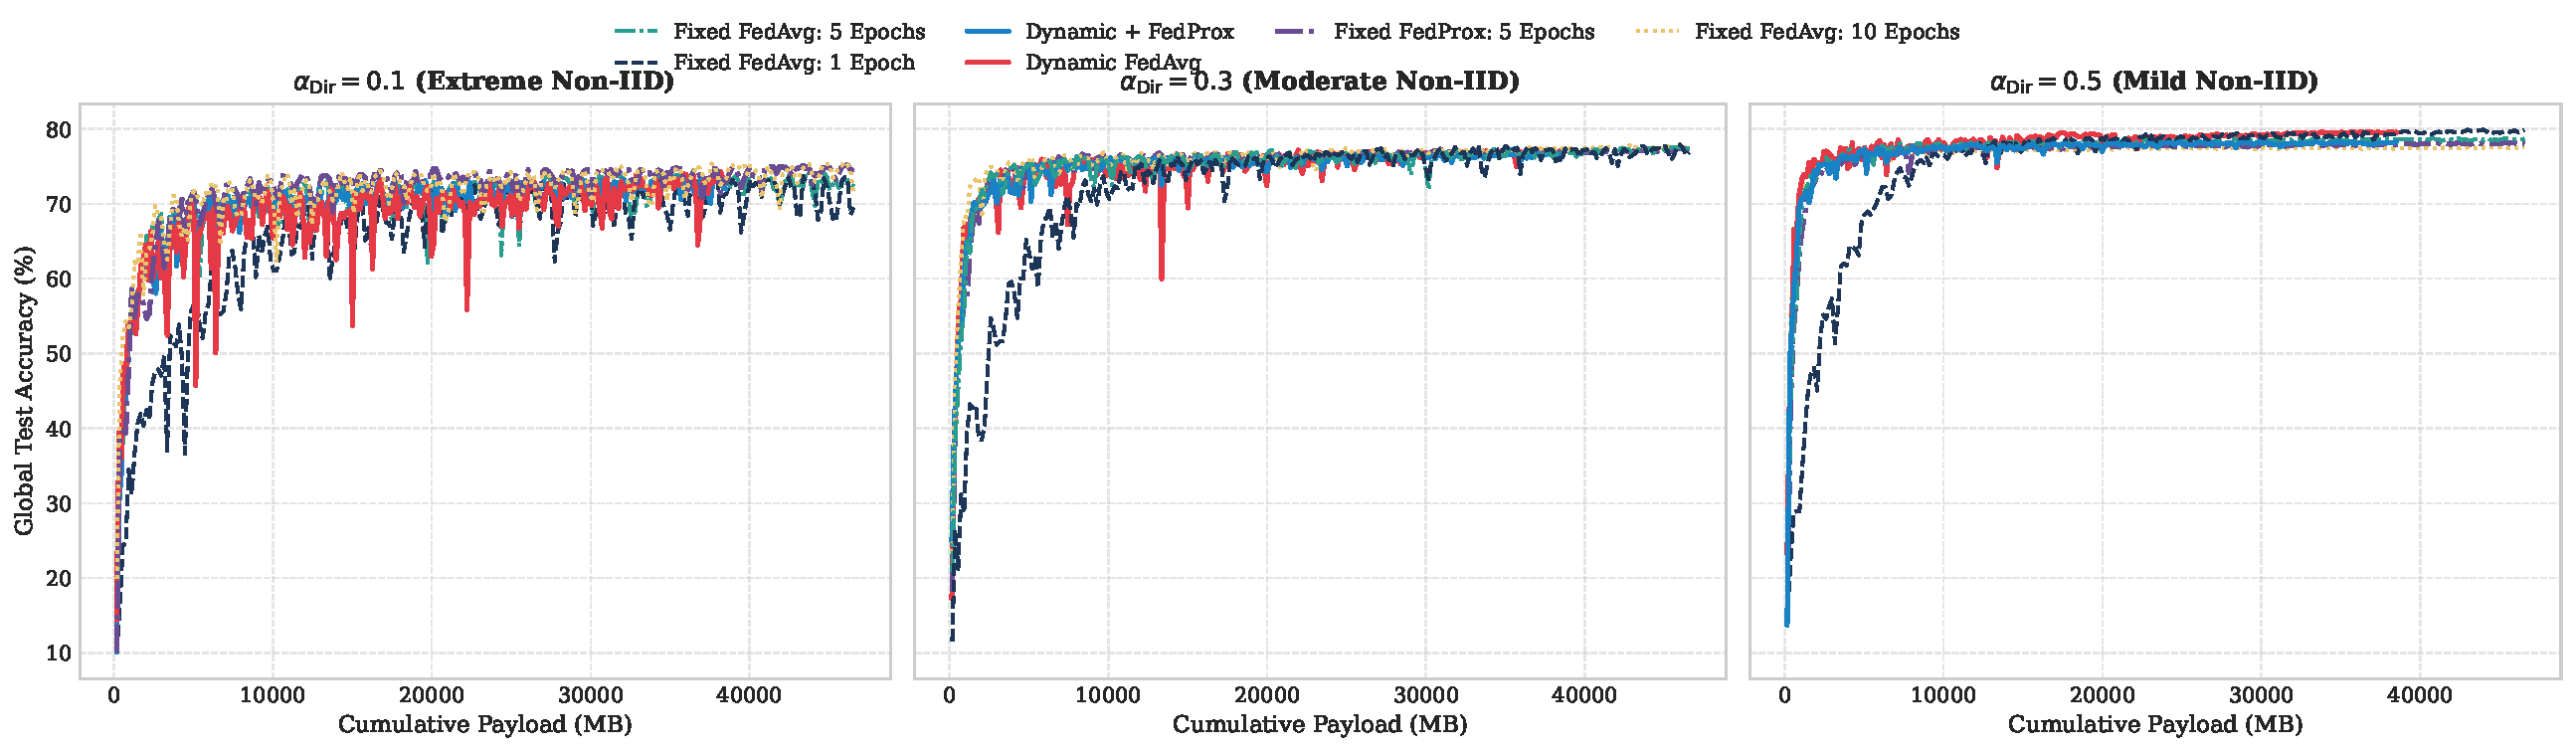
\includegraphics[width=0.98\linewidth]{plots/fig1_dirichlet_comparison.pdf}
\caption{Global centralized test accuracy (\%) plotted against cumulative transmitted model payload (MB) across non-IID Dirichlet partitioning regimes ($\alpha_{\text{Dir}} \in \{0.1, 0.3, 0.5\}$).}
\label{fig:accuracy_vs_mb}
\end{figure*}

\begin{figure}[t]
\centering
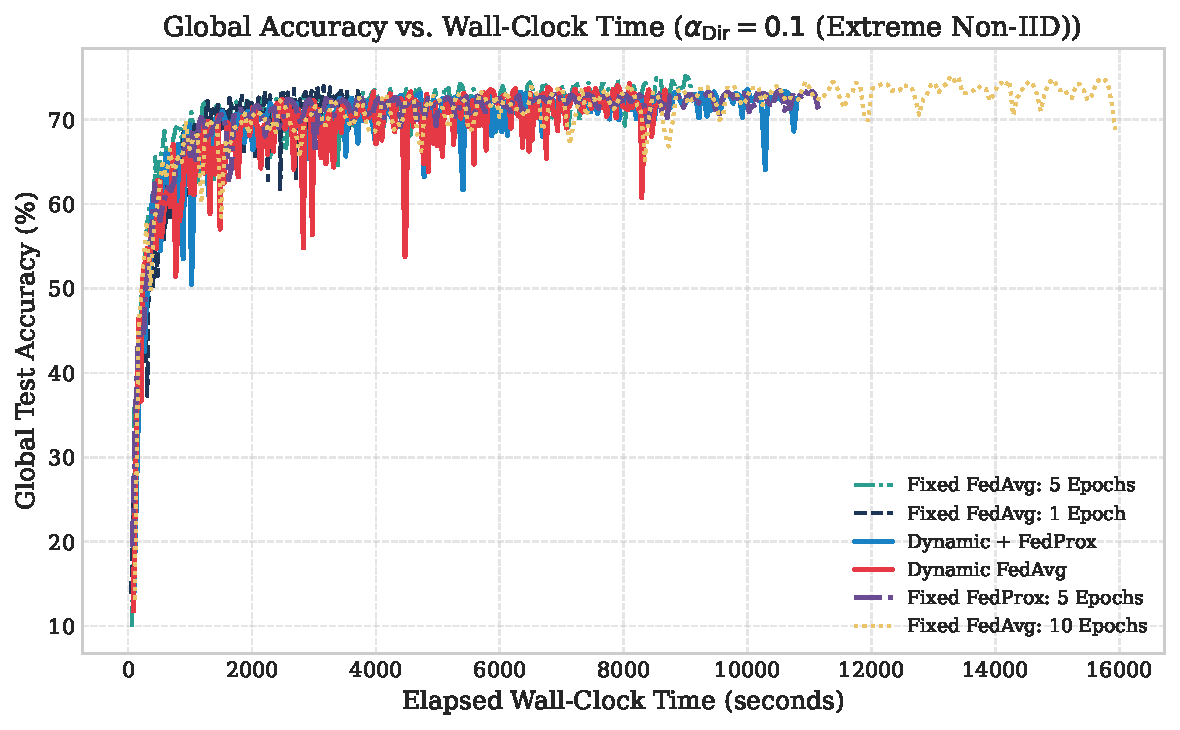
\includegraphics[width=0.92\linewidth]{plots/fig2_accuracy_vs_wall_time.pdf}
\caption{Global validation accuracy (\%) as a function of elapsed wall-clock execution time (seconds).}
\label{fig:accuracy_vs_time}
\end{figure}

\subsection{Communication Efficiency vs. Global Accuracy}
Table~\ref{tab:evaluation_results} and Figure~\ref{fig:accuracy_vs_mb} summarize global model convergence across extreme ($\alpha_{\text{Dir}} = 0.1$), moderate ($\alpha_{\text{Dir}} = 0.3$), and mild ($\alpha_{\text{Dir}} = 0.5$) non-IID data distributions. A fundamental bottleneck in vehicular federated learning is the asymmetry and scarcity of V2I uplink capacity: while base stations can broadcast global models across broad downlink channels, vehicle-to-infrastructure uploads are constrained by physical cell bandwidth and dynamic channel fading. Static scheduling frameworks ignore this physical limitation, forcing all sampled vehicles to attempt model uploads at every round. Over 250 rounds, static baselines accumulate 23,272.2~MB (23.3~GB) in raw uplink traffic (46,544.4~MB total bidirectional transmission) and trigger 567 buffer dropouts when vehicles attempt to upload through congested channels.

In contrast, our dynamic policy engine continuously monitors channel conditions and estimated local learning progress before permitting transmission. When links deteriorate, vehicles transition into \texttt{CONTINUE} or \texttt{WAIT}, keeping cumulative uplink transfers down to 15,238.6~MB. This achieves a 34.5\% reduction in pure uplink bandwidth consumption (saving over 8.0~GB of wireless transmissions, and a 17.3\% reduction in total bidirectional data) while slashing buffer dropouts by 83.2\% (from 567 to 95).

Crucially, these bandwidth savings do not impair convergence accuracy. Under extreme statistical heterogeneity ($\alpha_{\text{Dir}} = 0.1$), client datasets are heavily imbalanced. In this regime, Fixed FedAvg with $E=10$ overfits to skewed local partitions, causing parameter vectors to pull in contradictory directions and degrading aggregated centralized test accuracy to 68.87\%. Dynamic FedAvg attains 70.29\%, while pairing the dynamic scheduler with proximal regularization (Dynamic FedProx) achieves 72.51\%, outperforming Fixed $E=10$ (+3.64\%) and Fixed FedProx (+1.70\%). Under moderate and mild heterogeneity ($\alpha \in \{0.3, 0.5\}$), all methods reach comparable final accuracy (~76.5--77.6\% and ~78.1--78.8\%), yet the dynamic engine achieves this parity while expending one-third less uplink bandwidth and virtually eliminating upload failures.

Figure~\ref{fig:accuracy_vs_time} plots centralized test accuracy against elapsed wall-clock execution time. By bypassing congested transmission buffers and deferring training during peak safety-critical processor loads, dynamic vehicles avoid straggler delays and achieve steady wall-clock progress.

\begin{figure}[t]
\centering
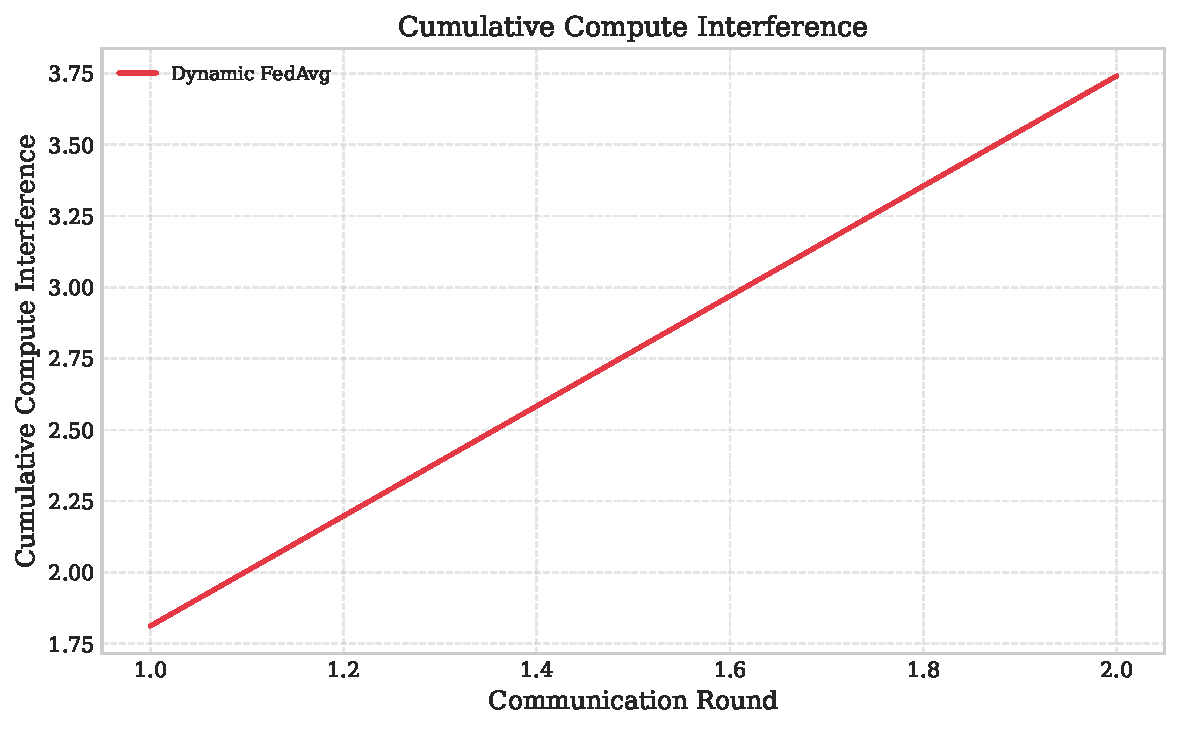
\includegraphics[width=0.92\linewidth]{plots/fig3_cumulative_compute_interference.pdf}
\caption{Cumulative compute interference imposed on safety-critical vehicular workloads across communication rounds.}
\label{fig:compute_interference}
\end{figure}

\begin{figure*}[t]
\centering
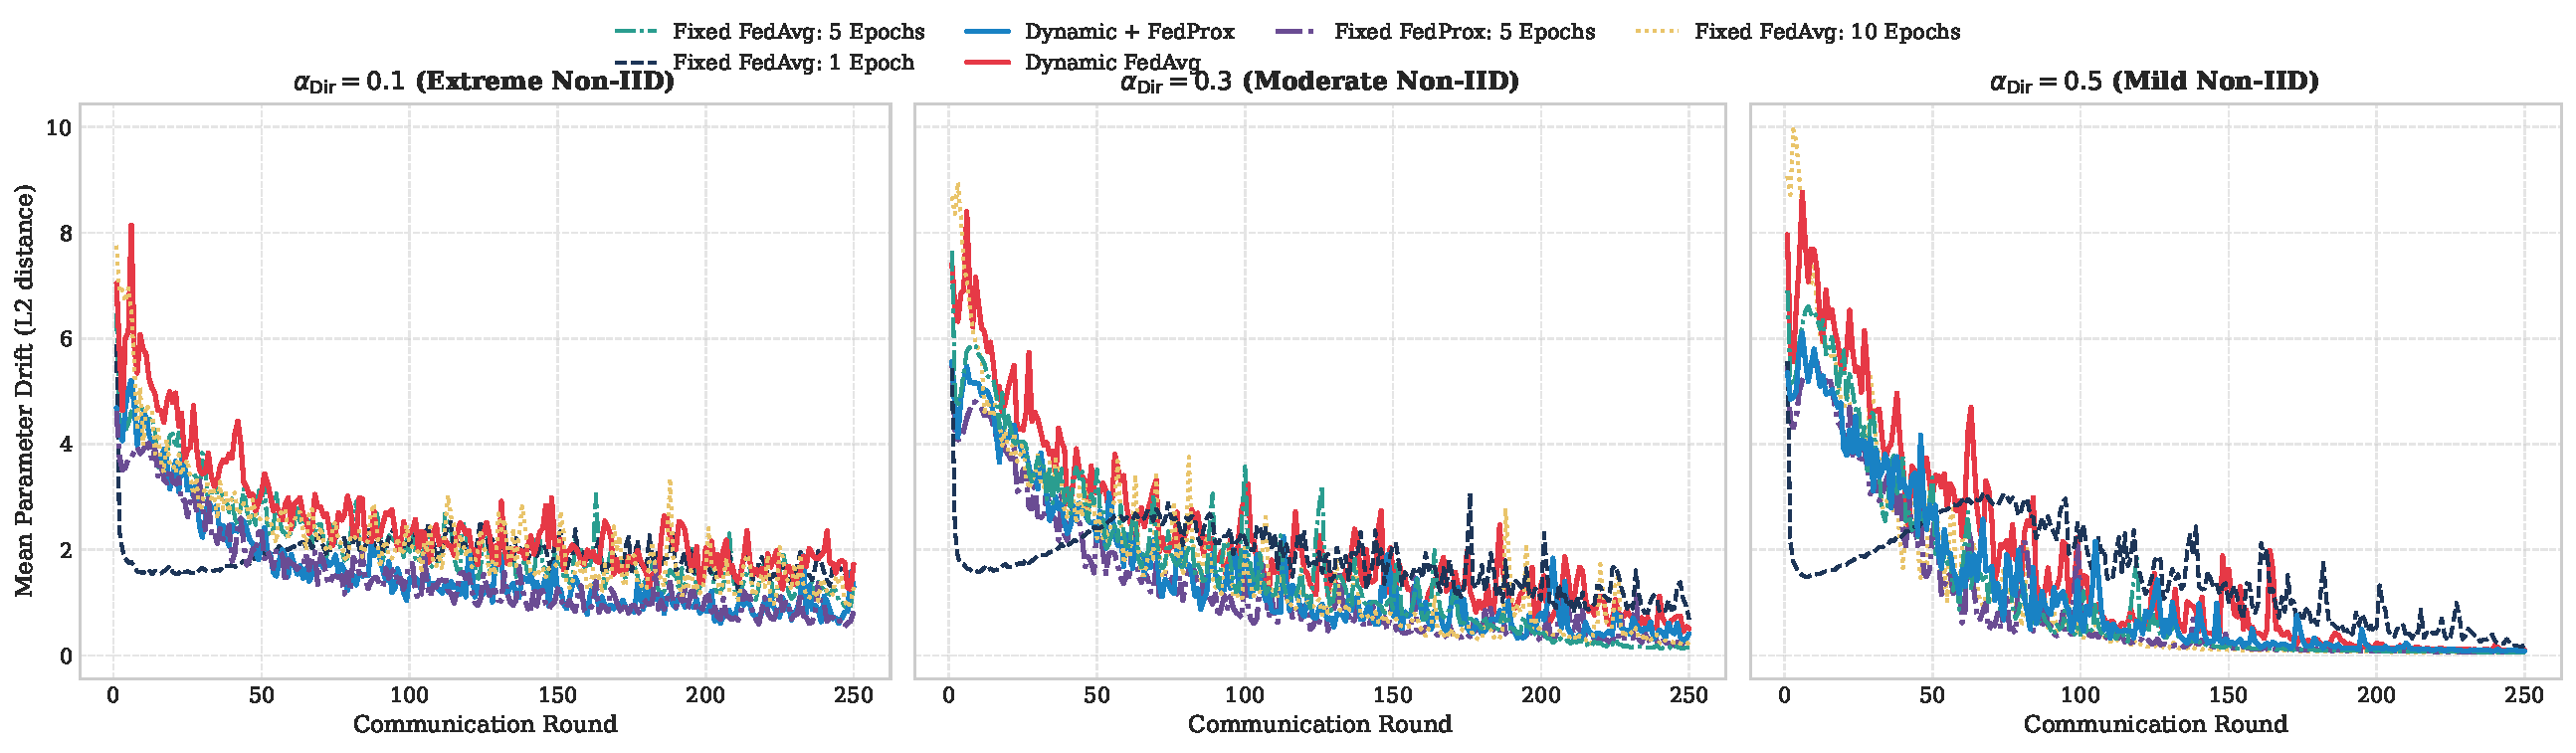
\includegraphics[width=0.98\linewidth]{plots/fig4_dirichlet_drift_comparison.pdf}
\caption{Mean client parameter divergence ($D_i(t) = \|\mathbf{w}_i - \mathbf{w}_{\text{global}}\|_2$) across communication rounds for $\alpha_{\text{Dir}} \in \{0.1, 0.3, 0.5\}$.}
\label{fig:model_drift}
\end{figure*}

\begin{figure}[t]
\centering
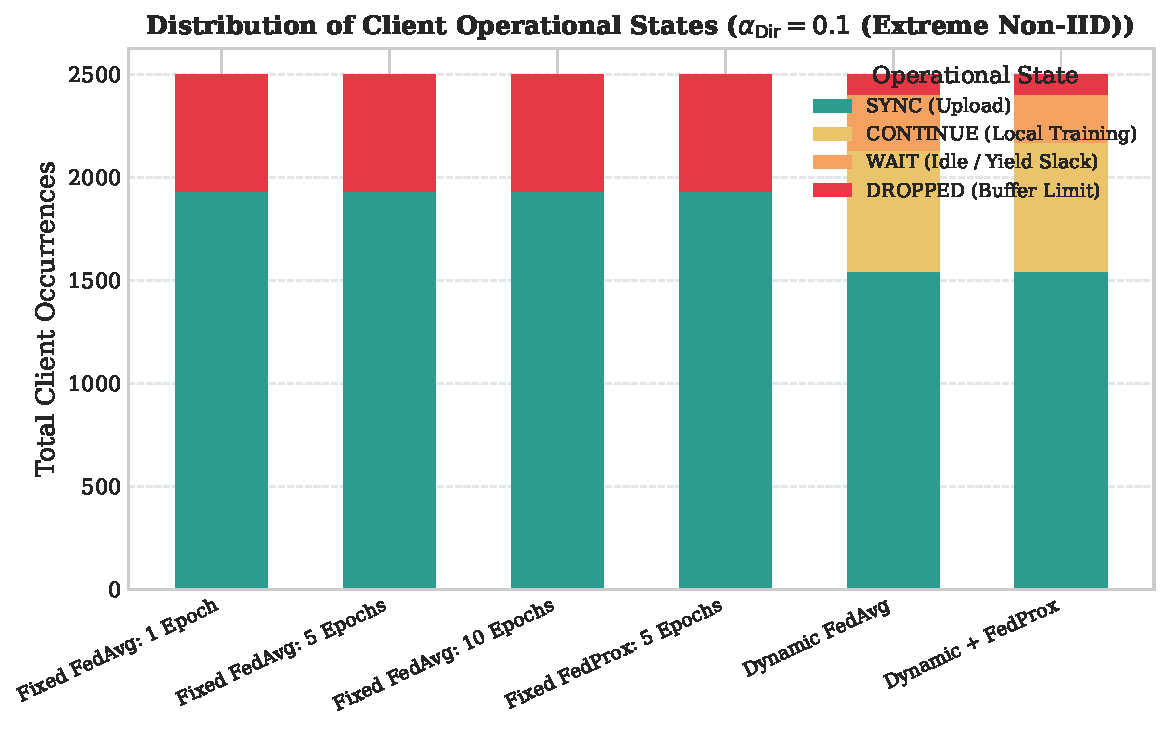
\includegraphics[width=0.92\linewidth]{plots/fig5_client_state_distribution.pdf}
\caption{Distribution of client operational states across the 250-round simulation ($\alpha_{\text{Dir}} = 0.1$). Static regimes blindly trigger 567 buffer dropouts under channel bottlenecks, whereas the dynamic engine redirects clients into autonomous local training (\texttt{CONTINUE}) and idle compute yielding (\texttt{WAIT}).}
\label{fig:client_states}
\end{figure}

\subsection{Compute Contention and Model Drift Analysis}
Figure~\ref{fig:compute_interference} compares cumulative compute interference on safety-critical vehicular workloads ($\sum c_i(t) U_i^{\text{crit}}(t)$). Static policies schedule local epochs without regard for co-located processor occupancy. Consequently, Fixed $E=10$ accumulates severe contention (1,000.6) and Fixed $E=5$ reaches 500.3, repeatedly training through periods when high ADAS processor demands leave minimal execution headroom. In contrast, our policy engine enforces an active compute slack threshold ($\text{slack} \ge 2.0/\rho_i$): whenever safety workload occupancy exceeds 80\% ($U_i^{\text{crit}} > 0.8$), training yields execution slack to background perception tasks. This keeps cumulative compute contention bounded between 373.0 and 398.5 across all non-IID regimes---a 60.7\% reduction compared to Fixed $E=10$ and a 21.4\% reduction compared to Fixed $E=5$.

Figure~\ref{fig:model_drift} illustrates client model drift measured via true parameter vector Euclidean distance across communication rounds. High-epoch static regimes allow local weights to diverge substantially under non-IID skew (accumulating 4,309.7 in drift under $\alpha=0.1$ for $E=10$), resulting in destructive parameter interference upon federated averaging. Dynamic FedProx curtails cumulative drift to 2,541.1 under $\alpha=0.1$ and 2,038.3 under $\alpha=0.5$---a 41.0\% drift reduction compared to Fixed $E=10$---by combining bounded utility checks that truncate unpromising epochs with proximal regularization that anchors updates to global parameters.

\subsection{Client Operational State Dynamics}
Figure~\ref{fig:client_states} illustrates how vehicular clients distribute their execution across operational states over the 250-round simulation. Under static regimes ($E \in \{1, 5, 10\}$ and FedProx), clients operate in a rigid binary pattern: attempting to upload parameter updates whenever sampled, which leads to 1,933 upload attempts and 567 transmission drops due to cell capacity bottlenecks.

In contrast, our dynamic engine actively exercises the three-state execution model. Across 2,500 client-round opportunities under severe skew ($\alpha_{\text{Dir}} = 0.1$), vehicles transitioned into \texttt{CONTINUE} 590 times and into \texttt{WAIT} 273 times. The 590 \texttt{CONTINUE} transitions represent intervals where channel throughput was inadequate for safe upload, but the vehicle predicted positive marginal loss reduction from continued local optimization. Because local weights persist on disk across simulation rounds, clients continued refining their models locally rather than forfeiting training progress. The 273 \texttt{WAIT} transitions represent critical safety and resource interventions: vehicles paused training because ADAS tasks required immediate processor capacity or because wireless conditions were poor and anticipated learning progress had plateaued. Consequently, upload dropouts dropped from 567 down to 95 (an 83.2\% reduction), transforming wasted network collisions into constructive, protected local learning.

\section{Conclusion}
This paper presented an online runtime policy engine for federated learning in Software-Defined Vehicles that addresses the fundamental trade-offs between mixed-criticality onboard compute demands and time-varying V2X wireless bandwidth. By coordinating client transitions across three discrete execution states (\texttt{WAIT}, \texttt{CONTINUE}, \texttt{SYNC}) using bounded loss extrapolation and real-time slack inspection, the engine ensures that vehicular learning progress neither starves safety-critical workloads nor overburdens the cellular uplink. Empirical evaluations across non-IID Dirichlet distributions demonstrate that the dynamic engine achieves convergence competitive with high-frequency synchronization regimes while reducing cumulative uplink bandwidth consumption by 34.5\%, slashing wireless transmission buffer dropouts by 83.2\%, and reducing compute interference on safety-critical tasks by up to 60.7\%. Future research will explore integration with vehicle trajectory prediction to proactively anticipate cellular handovers and examine 5G NR sidelink (V2V) cooperative parameter exchanges for distributed local aggregation.

\begin{thebibliography}{00}
\bibitem{ref_hong} Y. Hong, B. Lv, S. Wang, R. Wang, H. Tan, and F. C. Lau, ``Fedcars: An efficient scheduling framework for in-vehicle federated learning integrated with carla-cosimulation,'' \textit{IEEE Transactions on Vehicular Technology}, vol. 74, no. 5, pp. 7997--8011, 2025.
\bibitem{ref_karatas} M. Karatas et al., ``VR-VFL: Joint rate and client selection for vehicular federated learning under imperfect CSI,'' \textit{IEEE Transactions on Mobile Computing}, early access, 2026.
\bibitem{ref_yan} J. Yan, T. Chen, Y. Sun, Z. Nan, S. Zhou, and Z. Niu, ``Dynamic scheduling for vehicle-to-vehicle communications enhanced federated learning,'' \textit{IEEE Transactions on Wireless Communications}, pp. 9373--9390, 2024.
\bibitem{ref_qiang} X. Qiang, Z. Chang, Y. Hu, L. Liu, and T. H{\"a}m{\"a}l{\"a}inen, ``Adaptive and parallel split federated learning in vehicular edge computing,'' \textit{IEEE Internet of Things Journal}, vol. 12, no. 5, pp. 4591--4604, 2025.
\bibitem{ref_ballotta} L. Ballotta, N. D. Fabbro, G. Perin, L. Schenato, M. Rossi, and G. Piro, ``VREM-FL: Mobility-aware computation-scheduling co-design for vehicular federated learning,'' \textit{IEEE Transactions on Vehicular Technology}, vol. 74, no. 2, pp. 3311--3326, 2025.
\bibitem{ref_zhang_selection} X. Zhang, Z. Chang, T. Hu, W. Chen, X. Zhang, and G. Min, ``Vehicle selection and resource allocation for federated learning-assisted vehicular network,'' \textit{IEEE Transactions on Mobile Computing}, vol. 23, no. 5, pp. 3817--3829, 2024.
\bibitem{ref_pervej} M. F. Pervej, R. Jin, and H. Dai, ``Resource constrained vehicular edge federated learning with highly mobile connected vehicles,'' \textit{IEEE Journal on Selected Areas in Communications}, pp. 1825--1844, 2023.
\bibitem{ref_fedprox} T. Li, A. K. Sahu, M. Zaheer, M. Sanjabi, A. Talwalkar, and V. Smith, ``Federated optimization in heterogeneous networks,'' in \textit{Proc. MLSys}, 2020, pp. 429--450.
\bibitem{ref_liu} S. Liu, G. Yu, R. Yin, J. Yuan, and F. Qu, ``Communication and computation efficient federated learning for internet of vehicles with a constrained latency,'' \textit{IEEE Transactions on Vehicular Technology}, vol. 73, no. 1, pp. 1038--1052, 2024.
\bibitem{ref_zhang_quant} X. Zhang, W. Chen, H. Zhao, Z. Chang, and Z. Han, ``Joint accuracy and latency optimization for quantized federated learning in vehicular networks,'' \textit{IEEE Internet of Things Journal}, vol. 11, no. 17, pp. 28876--28890, 2024.
\bibitem{ref_wu} M. Wu, M. Boban, and F. Dressler, ``Flexible training and uploading strategy for asynchronous federated learning in dynamic environments,'' \textit{IEEE Transactions on Mobile Computing}, pp. 12907--12921, 2024.
\bibitem{ref_zhang_automotive} H. Zhang, J. Bosch, and H. H. Olsson, ``Real-time end-to-end federated learning: An automotive case study,'' in \textit{Proc. IEEE 45th Annual Computers, Software, and Applications Conference (COMPSAC)}, 2021, pp. 459--468.
\end{thebibliography}

\end{document}